\subsection{Herramientas de OpenAI}

OpenAI tiene a disposición del público tres importantes herramientas de interacción con sus modelos de lenguaje (entre otros modelos). 

    \paragraph{ChatGPT.} Esta es, sin duda, la más conocida y utilizada por el gran público. Fue publicada en noviembre de 2022, y el crecimiento en número de usuarios fue en ese momento el más rápido de la historia de la tecnología. En la figura \ref{fig:crecimiento_chatgpt} se puede observar el crecimiento de usuarios en los primeros meses de vida de la herramienta. ChatGPT es una herramienta de interacción con el modelo GPT-3 y GPT-4 (este último modelo reservado a usuarios de ChatGPT Plus), que permite introducir texto y obtener una respuesta del modelo. La respuesta puede ser de tipo textual, o bien de tipo visual, en forma de imagen, utilizando para ello el modelo de generación de imágenes DALL-E 3. La herramienta está disponible en la web de OpenAI, y se puede acceder a ella tanto a través de un navegador web como de una aplicación móvil.

    Esta interfaz de comunicación con los \gls{llm} de OpenAI tiene diversas modalidades de uso. Por una parte, se puede utilizar como un chat convencional, en el que se introduce texto y se obtiene una respuesta, pudiendo elegir el modelo de lenguaje entre GPT-3 y GPT-4. En noviembre de 2023 OpenAI lanzó lo que ha venido a denomiar GPTs, que no son otra cosa que chats que contienen un prompt predefinido por el usuario, así como la posibilidad de consulta de documentos subidos por este. En la figura \ref{fig:chatgpt} se puede observar la interfaz de ChatGPT en modo chat.

    \begin{figure}[h]
        \caption[Crecimiento de ChatGPT]{Crecimiento de ChatGPT}
        \centering
        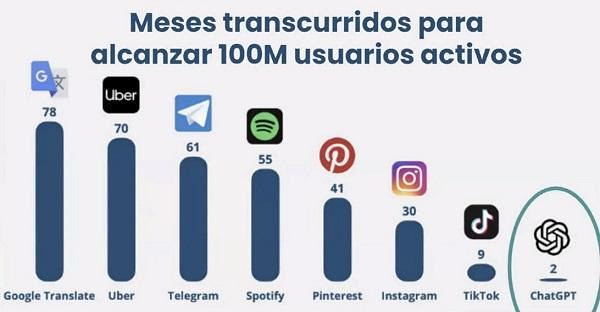
\includegraphics[width=0.6\textwidth]{./figuras/100millonesUsuariosChatgpt.jpeg}
        \source{\cite{PrimerosMesesChat2023}}
        \label{fig:crecimiento_chatgpt}
    \end{figure}

    \begin{figure}[h]
        \caption[Interfaz web de ChatGPT]{Interfaz web de ChatGPT}
        \centering
        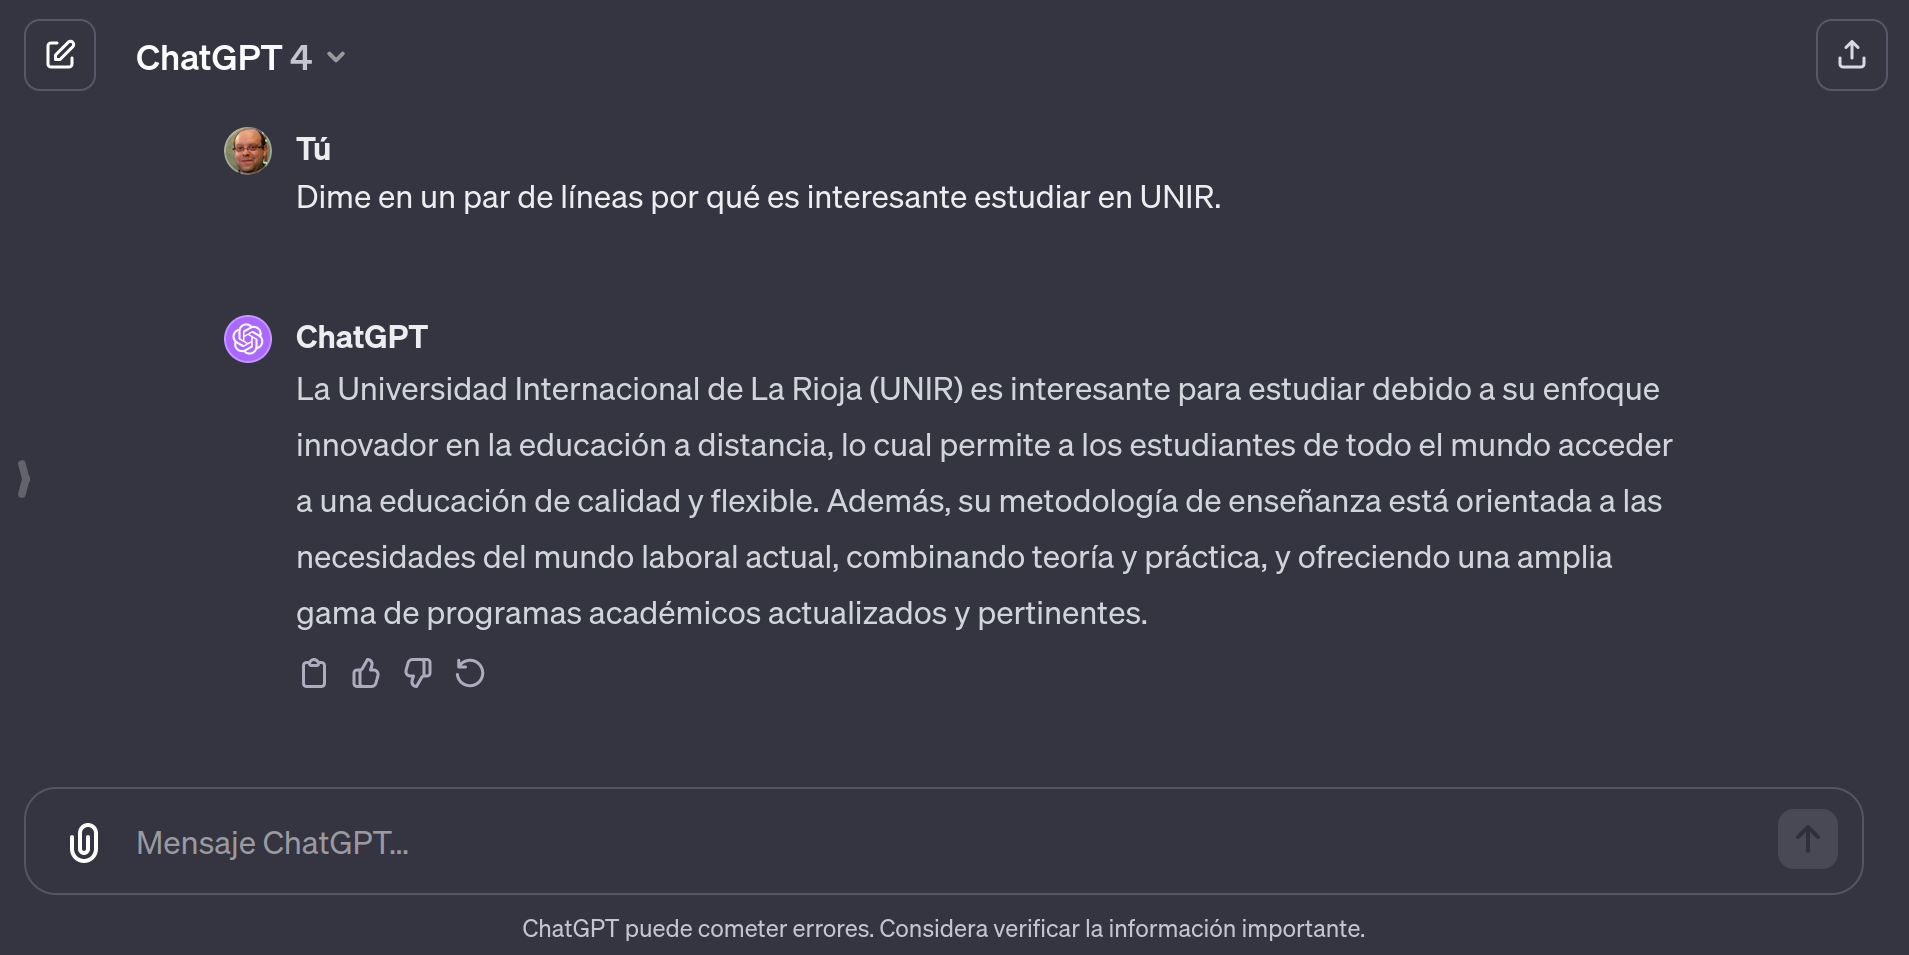
\includegraphics[width=0.7\textwidth]{./figuras/interfaz_chatgpt.png}
        \source{\propio}
        \label{fig:chatgpt}
    \end{figure}

    \paragraph{\emph{Playground.}} Esta herramienta permite interactuar con los modelos de lenguaje de OpenAI de forma más flexible que ChatGPT. En ella se pueden introducir \emph{prompts} de texto, así como seleccionar el modelo de lenguaje a utilizar, el número de respuestas a obtener, la \emph{temperatura} de generación, la presencia o ausencia de \emph{stopwords}, y la presencia o ausencia de \emph{top\_p sampling}, todos ellos parámetros avanzados en la interacción con los \gls{llm} (véase \ref{sec:hiperparametros_controlables}), sobre los que no existe ningún control por parte del usuario en la versión web de chatGPT. En la figura \ref{fig:playground} se puede observar la interfaz de Playground, donde el usuario puede introducir un \emph{prompt} de sistema, así como un mensaje de usuario, y obtener una respuesta del modelo de acuerdo a los parámetros seleccionados de \emph{temperatura} y \emph{top\_p sampling}. Esta herramienta es muy útil para la experimentación de esta y otras investigaciones con \gls{llm}, ya que permite una interacción más flexible con los \gls{llm}.

    \begin{figure}[h]
        \caption[Interfaz de \emph{Playground} de OpenAI]{Interfaz de \emph{Playground} de OpenAI}
        \centering
        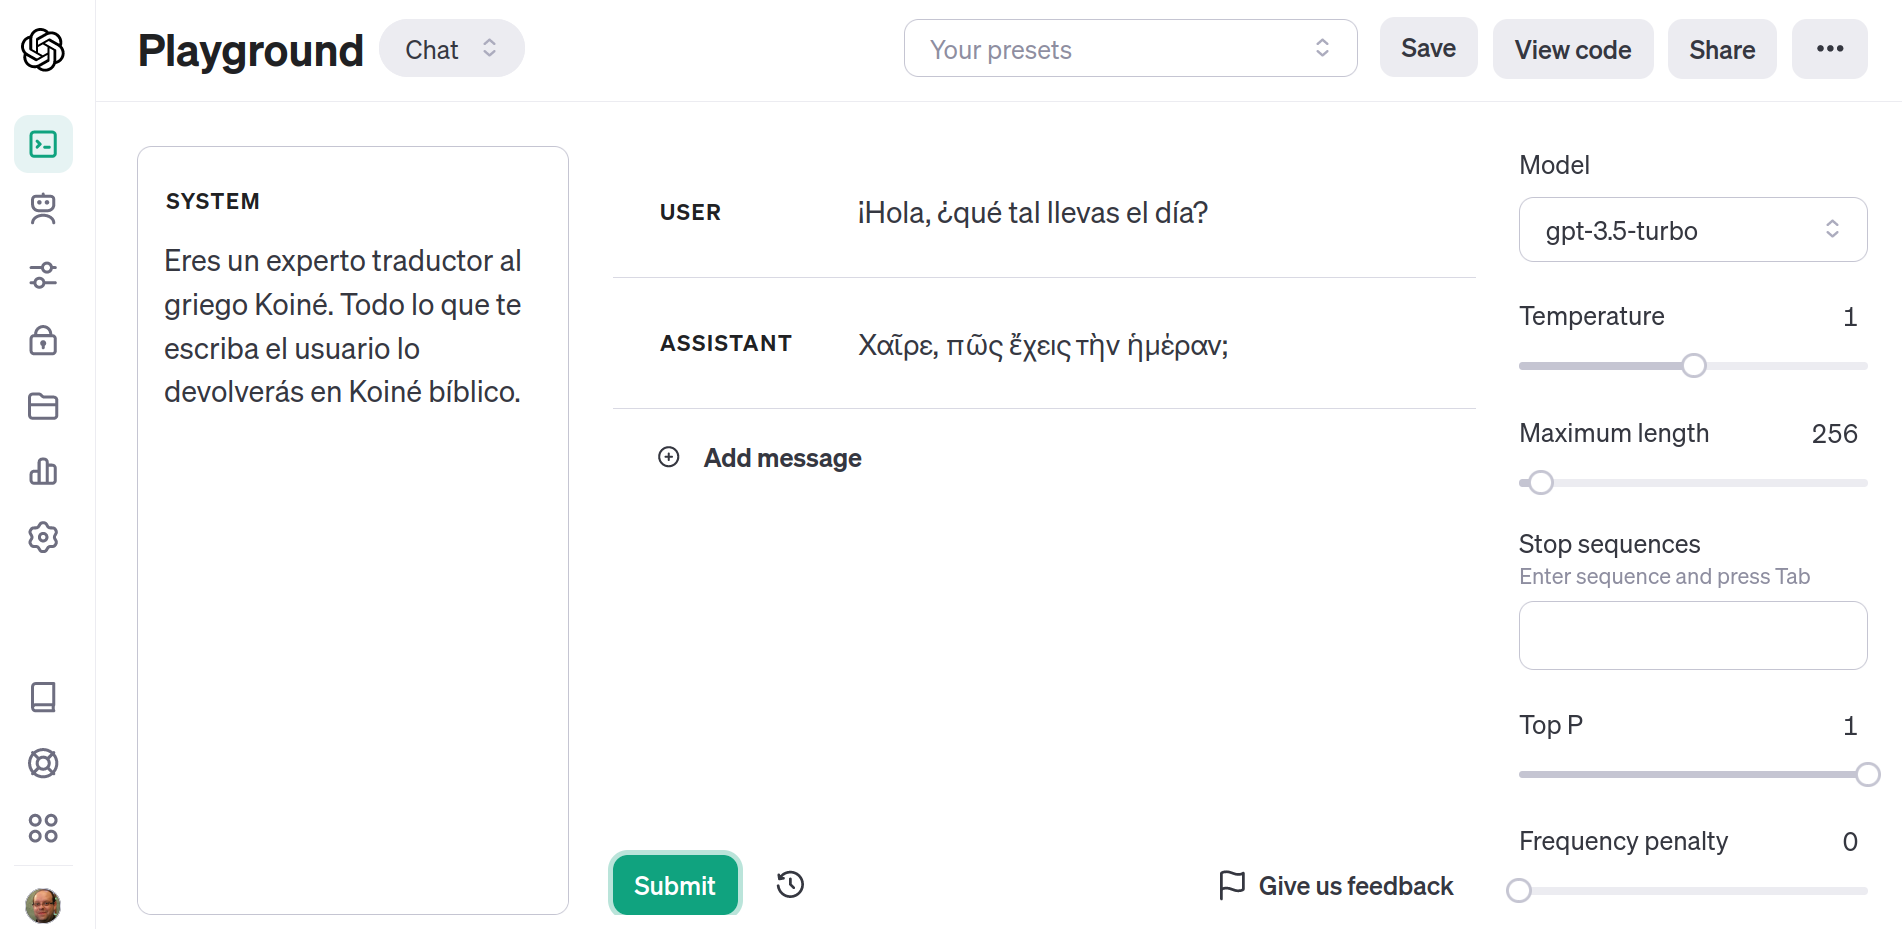
\includegraphics[width=0.7\textwidth]{./figuras/interfaz_playground.png}
        \source{\propio}
        \label{fig:playground}
    \end{figure}

    \paragraph{\gls{api} de OpenAI.} La herramienta \emph{Playground} no es sino la antesala de la \gls{api} de OpenAI. \glsdisp{api}{\emph{Aplication programming interface}} es un conjunto de funciones y procedimientos que ofrece una biblioteca para ser utilizado por otro software como una capa de abstracción. En el caso de OpenAI, la \gls{api} permite la interacción con los \gls{llm} de forma programática, es decir, mediante código. Esto permite una interacción absolutamente flexible a la par que potente con los \gls{llm}, ya que se pueden automatizar procesos, y se puede interactuar con los \gls{llm} de forma más rápida y eficiente. La \gls{api} de OpenAI permite la interacción con diversos modelos de lenguaje basados en GPT-3 y GPT-4, así como con el modelo de generación de imágenes DALL-E 3. En la figura \ref{fig:api} se puede observar un ejemplo de interacción con la \gls{api} de OpenAI, en el que se introduce un \emph{prompt} de sistema, otro de usuario, se ajustan los hiperparámetros y se obtiene una respuesta del modelo.

    \begin{figure}[h]
        \caption[Ejemplo con \gls{api} de OpenAI]{Ejemplo con \gls{api} de OpenAI}
        \centering
        \includegraphics[width=0.7\textwidth]{./figuras/ejemplo_\gls{api}.png}
        \source{\propio}
        \label{fig:api}
    \end{figure}

\subsection{Python como lenguaje de programación}
El uso de la \gls{api} de OpenAI requiere el uso de un lenguaje de programación. En este caso, se ha utilizado Python, un lenguaje de programación de propósito general, interpretado, de alto nivel y de tipado dinámico. Python es un lenguaje de programación muy popular, y es utilizado por la mayoría de los investigadores en el campo de la inteligencia artificial. Además, es un lenguaje de programación muy flexible, que permite la interacción con la \gls{api} de OpenAI de forma sencilla y eficiente. La propia OpenAI ofrece una biblioteca de Python para la interacción con su \gls{api}, que facilita la interacción con los \gls{llm}, así como una gran documentación y ejemplos de uso. 

Debido al amplio uso de Python como lenguaje de \emph{Deep Learning}, muchos de estos códigos se pueden compartir y ejecutar en servidores remotos, lo cual permite un trabajo con un flujo de trabajo distribuido entre varios investigadores. En el caso de el presente estudio,con el fin de realizar una sencilla interacción de la \gls{api} con los motores de sonido (SuperCollider y Tidal Cycles), se han programado todos los scripts para ser ejecutados en local.




% ---------





Para llevar a cabo la experimentación en esta investigación, se utilizará el modelo GPT-4 proporcionado por OpenAI a través de su \gls{api}. GPT-4 es, en el momento en que se escribe este texto, el modelo de lenguaje a gran escala más avanzado y potente disponible públicamente. Esta elección garantiza la interacción con una tecnología de vanguardia en el campo del procesamiento del lenguaje natural y el \emph{Deep Learning}. La \gls{api} de OpenAI permite una interacción flexible y eficiente con el modelo, facilitando la introducción de \emph{prompts} y la recopilación de respuestas en tiempo real.